\documentclass[tikz,border=3.14mm]{standalone}
\usetikzlibrary{backgrounds,calc,arrows,patterns,patterns.meta,calc,math}
\usepackage{pgfplots}
\pgfplotsset{compat=1.18}

\begin{document}
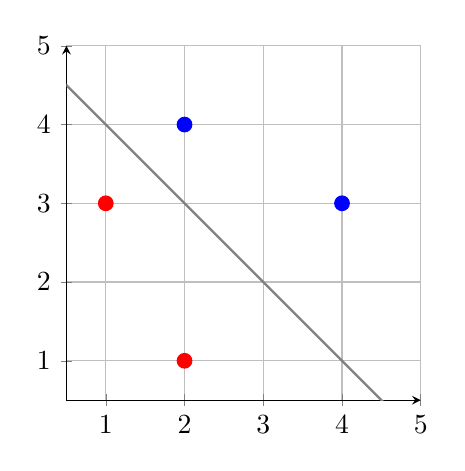
\begin{tikzpicture}[x=1cm,y=1cm]
    \begin{axis}[
        x=1.0cm,y=1.0cm,
        axis lines=middle,
        ymajorgrids=true,
        xmajorgrids=true,
        xmin=0.5,
        xmax=5.0,
        ymin=0.5,
        ymax=5.0,
        xtick={1.0,...,5.0},
        ytick={1.0,...,5.0}]
		\foreach \aaaa/\bbbb in {1/3,2/1} {
			\edef\temp{\noexpand\fill[red] (\aaaa,\bbbb) circle (0.1);}
			\temp
		}
		\foreach \aaaa/\bbbb in {2/4,4/3} {
			\edef\temp{\noexpand\fill[blue] (\aaaa,\bbbb) circle (0.1);}
			\temp
		}
		\draw[thick,gray] (0,5) -- (5,0);
	\end{axis}
\end{tikzpicture}
\end{document}
